\subsection{Pianificazione}
La pianificazione del percorso per i robot è uno dei criteri importanti da
prendere in considerazione per migliorare il livello di autonomia del robot.
Nella pianificazione del percorso, la sicurezza è un problema importante che 
dovrebbe essere preso in considerazione al fine di garantire che un robot 
raggiunga la posizione target senza collisioni con gli ostacoli circostanti.
Inoltre, ci sono aspetti importanti che devono essere affrontati nella 
pianificazione del percorso; tempo computazionale, percorso ottimale e 
completezza. 
Uno dei metodi più diffusi per la pianificazione dei percorsi è il metodo 
\emph{Campi Potenziali Artificiali}. 
Il metodo del potenziale è in grado di superare uno scenario sconosciuto, 
tenendo conto della realtà dell'ambiente corrente e del movimento del robot. 
Due tipi di forze sono coinvolte nel metodo del campo potenziale; forza attrattiva 
generata da obiettivi e forza repulsiva generata da ostacoli, di conseguenza, 
il robot deve riprogrammare un nuovo percorso\cite{apotetianfield}.
Utilizzando informazioni parziali sullo spazio di lavoro raccolte attraverso i 
sensori quindi le informazioni sensoriali sono integrate in una mappa secondo un 
paradigma \emph{sense---plan---move}.
Oppure utilizzare le informazioni sensoriali impiegate per pianificare moti 
secondo un paradigma \emph{stimulus---response} (navigazione reattiva).
Il robot è considerato come un punto sotto l'influenza dei campi prodotti da 
obiettivi e ostacoli nello spazio di ricerca. Le forze repulsive sono generate 
da ostacoli mentre la forza attrattiva è generata dagli obiettivi. La forza 
risultante (la somma di tutte le forze) dei campi sul robot viene utilizzato 
per determinare la direzione del movimento e la velocità di spostamento evitando 
collisioni\cite{5498220}.
Tuttavia esistono svantaggi quali:
\begin{enumerate*}[label={\alph*)},font={\bfseries}]
\item situazione di stallo dovuta ai minimi locali; 
\item oscillazione in presenza di ostacoli; 
\item nessun passaggio tra ostacoli ravvicinati; 
\item oscillazioni in passaggi stretti\cite{131810}.
\end{enumerate*}
Il robot viene considerato come punto $\mathbf{q} = (x \, y)^T$, in un piano 
cartesiano, attratto (potenziale $U_{\text{att}}$) dal punto obiettivo 
$\mathbf{q}_g$ e respinto (potenziale $U_{\text{rep}}$) dagli ostacoli.
\begin{equation}
\label{eq:apfm}
U(q) = U_{\text{att}}(q) + U_{\text{rep}}(q)
\end{equation}
%
\noindent dove $U(q)$ potenziale artificiale; $U_{\text{att}}(q)$ campo 
attrattivo; $U_{\text{rep}}(q)$ campo repulsivo.
La pianificazione avviene in modo incrementale: ad ogni configurazione 
$\mathbf{q}$, la forza artificiale viene generata come nell'equazione (\ref{eq:attractive}):
\begin{equation}
\label{eq:attractive}
\begin{split}
F(q) &= - \nabla U(q)\\
&= - \nabla U_{\text{att}}(q) -U_{\text{rep}}(q)\\
F(q) &= F_{\text{att}}(q) + F_{\text{rep}}(q)	
\end{split}
\end{equation}
dove $F(q)$: forza artificiale; $F_{\text{att}}(q)$: forza attrattiva; 
$F_{\text{rep}}(q)$: forza repulsiva. Il campo potenziale $U_{\text{att}}$) tra 
robot e obiettivo viene descritto da (\ref{eq:fieldattractive}) per trascinare 
il robot nell'area obiettivo.
\begin{equation}
\label{eq:fieldattractive}
\begin{split}
U_{\text{att}}(q) &= \frac{1}{2} \, k_a \, (q-q_d)^2\\
&= \frac{1}{2} \, k_a \, \rho^{2}_{goal}(q)
\end{split}
\end{equation}
dove $k_a$: coefficiente positivo per APF\footnote{Artificial Potential Field};
$q$: posizione corrente del robot; $q_{d}$: posizione corrente dell'obiettivo.
$\rho_{\text{goal}}(q) = \|q-q_{d}\|$ è una distanza euclidea dalla posizione 
del robot alla posizione dell'obiettivo. La forza attrattiva del robot è 
calcolata come gradiente negativo del potenziale campo\cite{6283526}:
\begin{equation}
\label{eq:gradientfield}
\begin{split}
F_{\text{att}}(q) &= -\frac{1}{2}k_a \rho^2_{\text{goal}}(q)\\
F_{\text{att}}(q) &= -k_a \, (q-q_d)
\end{split}
\end{equation}
%
$F_{\text{att}}(q)$, nell'eq. (\ref{eq:gradientfield}), è un vettore diretto 
verso $q_{\text{d}}$ con intensità linearmente proporzionale alla distanza da 
$q$ a $q_{\text{d}}$. Può essere scritto nelle sue componenti:
\begin{equation}
\label{eq:componet}
\begin{split}
F_{\text{att}} -x(q) &= -k_a \, (x - x_d)\\
F_{\text{att}} -y(q) &= -k_a \, (y - y_d)\\
\end{split}
\end{equation}
%
Le equazioni (\ref{eq:componet}) sono la forza attrattiva nelle direzioni $x$ 
e $y$. Nella funzione potenziale, il robot deve essere respinto dagli ostacoli, 
ma se lontano da questi, il movimento non risente della loro influenza.
La funzione potenziale di repulsione (\ref{eq:repulsive}) è:
\begin{equation}
\label{eq:repulsive}
U_{\text{rep}}(q) = 
\begin{cases} 
\frac{1}{2}k_b(\frac{1}{d(q)}-\frac{1}{d_0})^2 &\mbox{se } d(q) \leq d_0 \\ 
0 & \mbox{se } d(q) > d_0
\end{cases} 
\end{equation}
\begin{figure*}[htb]
\centering
\subfloat[][\emph{Campo attrattivo - repulsivo}.]
   {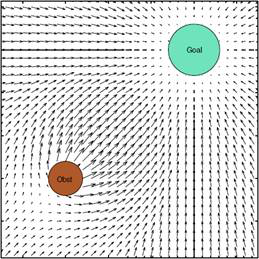
\includegraphics[width=.35\textwidth]{image008}} \quad
\subfloat[][\emph{Pianificazione traiettoria}.]
   {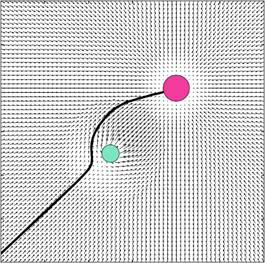
\includegraphics[width=.35\textwidth]{image010}} 
\caption{Potenziali artificiali}
\label{fig:potentialfield}
\end{figure*}
